\begin{figure}
\begin{fullwidth}
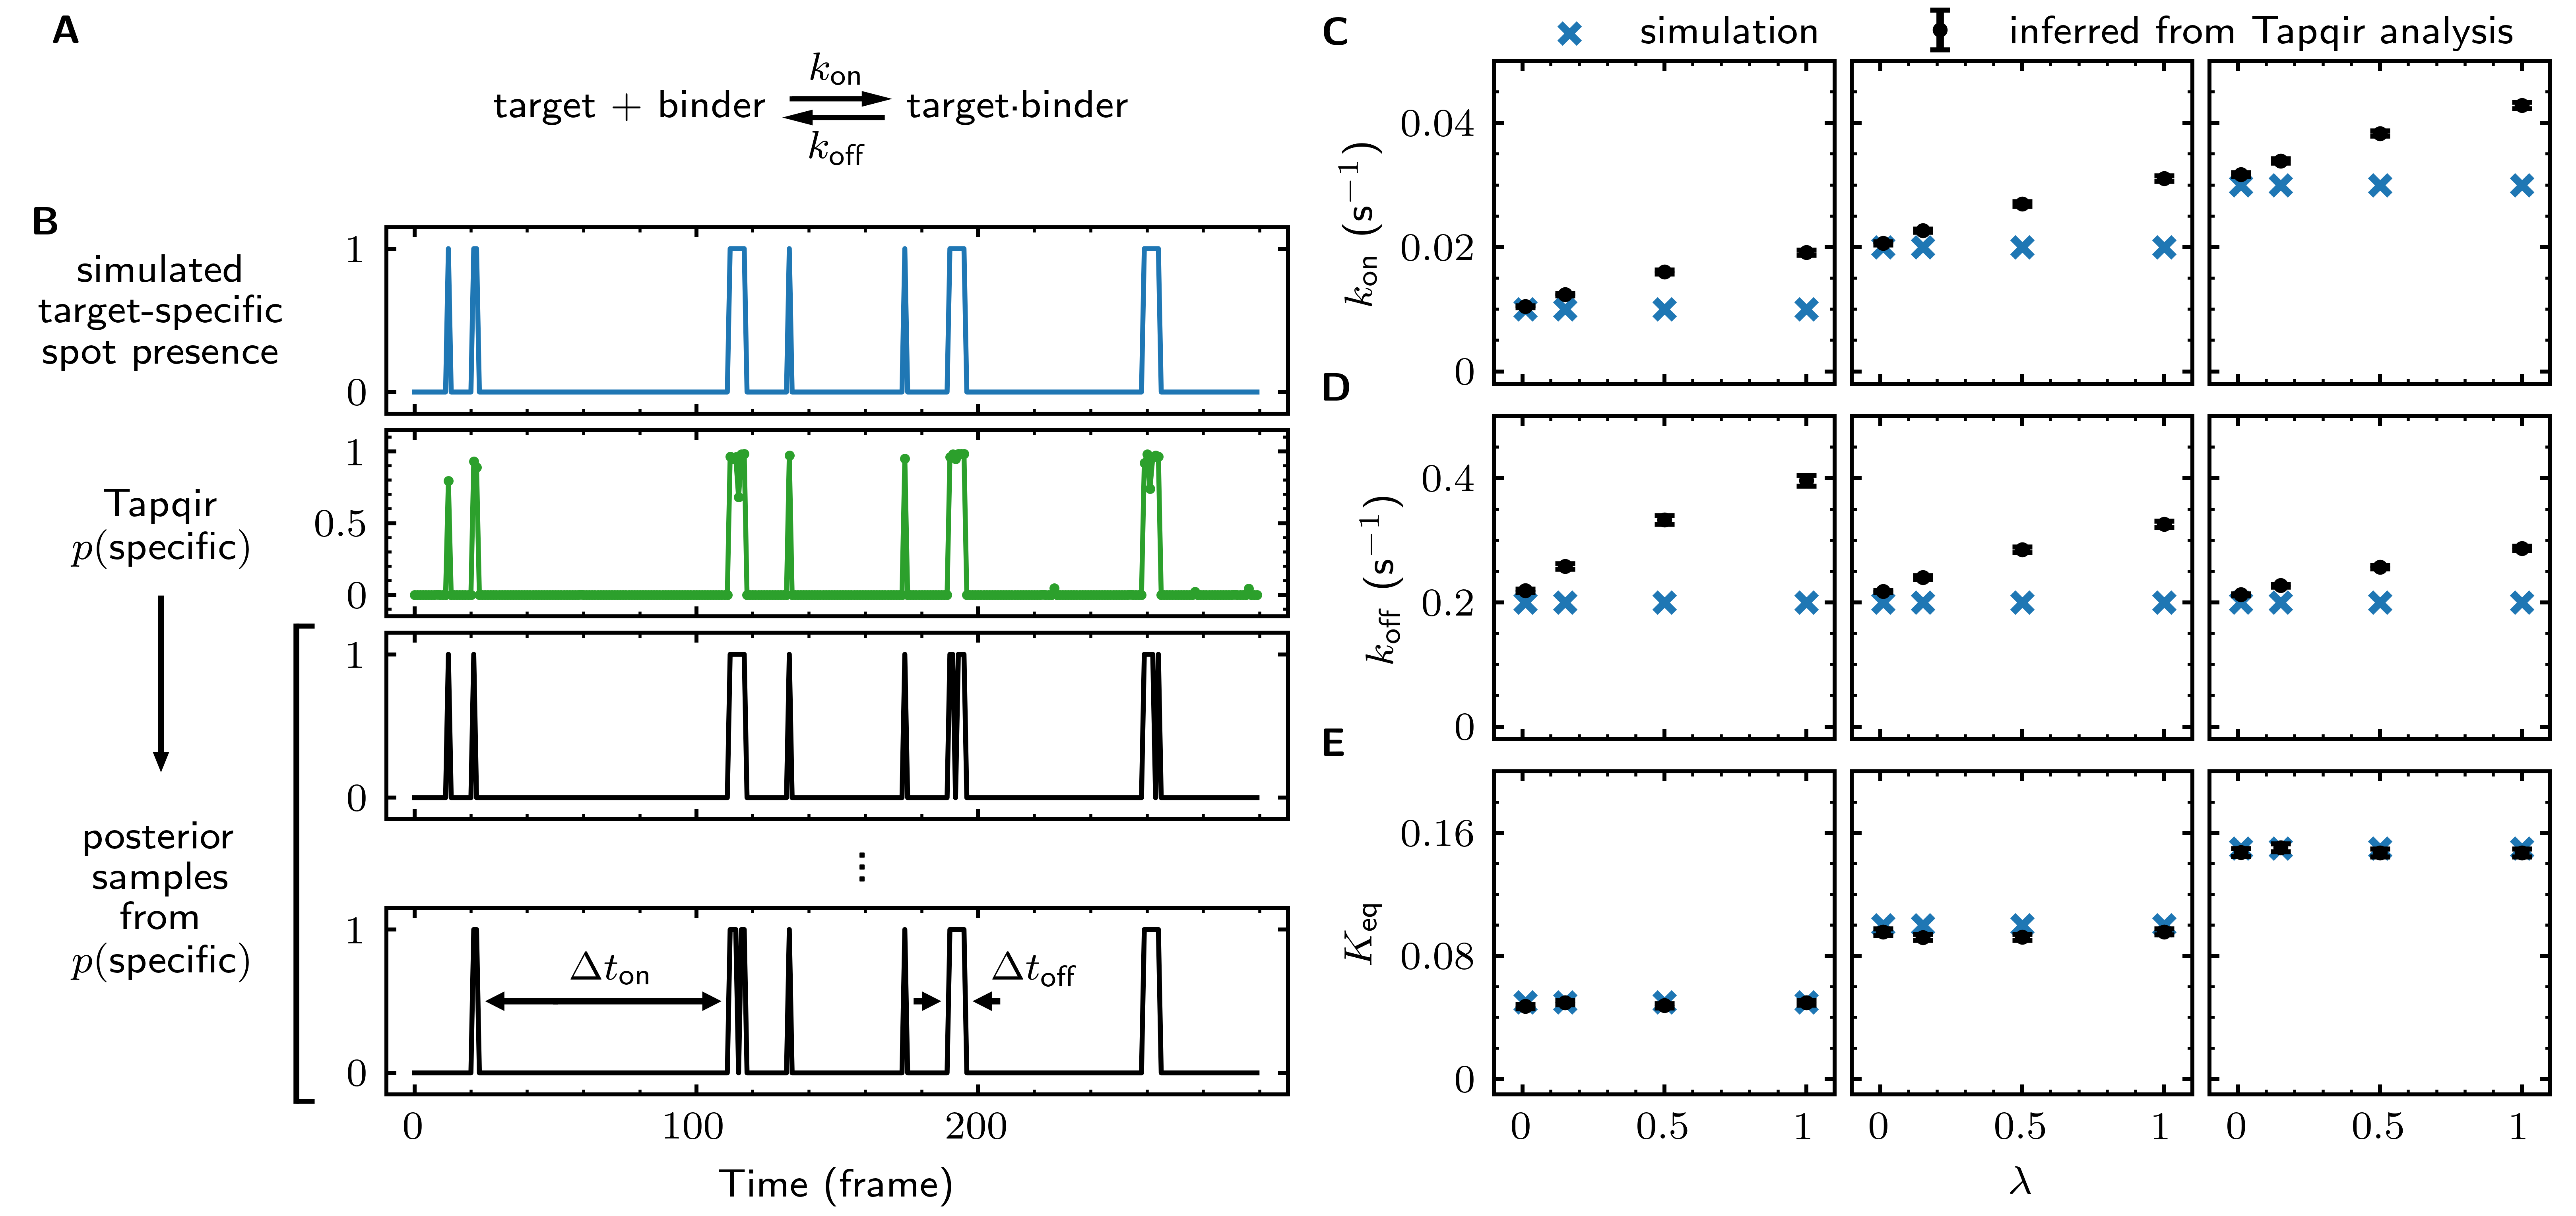
\includegraphics[width=183mm]{figures/kinetic_analysis.png}
\caption{\textbf{Tapqir analysis of association/dissociation kinetics and thermodynamics.} (\textbf{A}) Chemical scheme for a one-step association/dissociation reaction at equilibrium with apparent first-order binding and dissociation rate constants $k_{\mathsf{on}}$ and $k_{\mathsf{off}}$, respectively. (\textbf{B}) A simulation of the reaction in (\textbf{A}) and scheme for kinetic analysis with Tapqir. Simulation used SNR = 3.76, $k_\mathsf{on} = 0.02$ s$^{-1}$, $k_\mathsf{off} = 0.2$ s$^{-1}$, and a high target-nonspecific binding frequency $\lambda = 1$ (Supplemental Data 5, data set \texttt{kon0.02lamda1}). Full dataset consists of 100 AOI locations and 1000 frames each for on-target data and off-target control data. Shown is a short extract of on-target data from a single location in the simulation.  Plots show simulated presence/absence of the target-specific spot (blue) and Tapqir-calculated estimate of corresponding target-specific spot probability $p(\mathsf{specific})$ (green). Two thousand binary traces (e.g., black records) were sampled from the $p(\mathsf{specific})$ posterior distribution and used to infer $k_\mathsf{on}$ and $k_\mathsf{off}$ using a two-state hidden Markov model (HMM) (see Materials and Methods). Each sample trace contains well-defined time intervals corresponding to target-specific spot presence and absence (e.g., $\Delta t_\mathsf{on}$ and $\Delta t_\mathsf{off}$). (\textbf{C,D,E}) Kinetic and equilibrium constants from simulations (Supplemental Data 5) using a range of $k_\mathsf{on}$ values and  target-nonspecific spot frequencies $\lambda$, with constant $k_\mathsf{off} = 0.2$ s$^{-1}$. (\textbf{C}) Values of $k_{\mathsf{on}}$ used in simulations (blue) and mean values (and 95\% CIs, black) inferred by HMM analysis from the 2000 posterior samples.  Some error bars are smaller than the points and thus not visible. (\textbf{D}) Same as (\textbf{C}) but for $k_{\mathsf{off}}$. (\textbf{E})  Binding equilibrium constants $K_{\mathsf{eq}} = k_{\mathsf{on}} / k_{\mathsf{off}}$ used in simulation (blue) and inferred from Tapqir-calculated $\pi$ as $K_{\mathsf{eq}} = \pi / (1 - \pi)$ (black). }
\label{fig:kinetic_analysis}
\end{fullwidth}
\end{figure}